\documentclass[10.5pt,a4paper]{article}
\usepackage[utf8]{inputenc}
\usepackage{amsmath}
\usepackage{amsfonts}
\usepackage{amssymb}
\usepackage{graphicx}
\usepackage{setspace}
\usepackage{algorithm}
\usepackage{algpseudocode}
\usepackage{listings}
\usepackage{wrapfig}
\usepackage{hyperref}
\usepackage[left=1cm, right=1cm, top=1cm, bottom=2cm]{geometry}
\usepackage[font=small]{caption, subcaption}

%\setlength{\parskip}{0em}
\setstretch{0.3}

\algdef{SE}[SUBALG]{Indent}{EndIndent}{}{\algorithmicend\ }%
\algtext*{Indent}
\algtext*{EndIndent}

\newcommand{\algorithmautorefname}{Algorithm}

\begin{document}
    \begin{center}
        \large \textbf{Problem, Search and beyond}
        
        \normalsize Chuanyuna Liu 884140, Zhuoqun Huang 908525
    \end{center}
    \section{Problem}
    \subsection{General Problem}
    We formulate our problem with the following five concepts:
    \begin{itemize}
        \itemsep0em
        \item \textbf{State($\mathbb{S}$)} including a \textbf{initial state ($s_0$)} the agent begins with
        \item \textbf{Actions($\mathbb{A}$)} available to agent at each State
        \item \textbf{Transition function ($F:\mathbb{S}\times \mathbb{A}\rightarrow \mathbb{S}$)} that takes a (state, action) pair and return a new state
        \item \textbf{Goal Test($GT:S\rightarrow \{True, False\}$)} that takes a state $s$ and return true if $s\in S_{goal}$, the \textbf{Goal State} of the problem.
        \item \textbf{Path Cost ($C:\mathbb{S}\times \mathbb{S}\rightarrow \mathbb{R}$)} That takes two states and return cost moving from one to another
    \end{itemize}
    \vspace{-15pt}
    \subsection{Single-player Chexers}
    In this section, we formally describe how the above framework fits the Chexers game.
    \begin{itemize}
        \itemsep0em
        \item Denote set of pieces with $\mathbb{P}=\{(r, q, t)\}$. \\
        where
        \begin{align*}
            \text{$r, q, -(r+q)\in [-3, 3]$ denotes the location on board.}\\
            \text{$t\in \{red, blue, green, block\}$ stands for type of piece.}    
        \end{align*}
        
        \item $\mathbb{S} := \{p_i\in \mathbb{P}, t_b|i\le n\}$ where $n$ is number of pieces on board, where $t_b$ is the searching type.*
        \item $\mathbb{A} := \{(Move,p_i), (Jump, p_i), (Exit, p_i)\}, \forall\ p_i $ where$\ t(p_i)=t_b. | \mathbb{A}_s| \le 6n_p\ \forall s$.
        \item $f(s, a) := s'$. where $s'$ differs exactly by one piece $r(p_{i,s}), q(p_{i,s}) \ne r(p_{i,s'}), q(p_{i,s'})$ or $p_i\notin s'$
        \item $c(s, s') := 1, \forall s, s'\ \text{if}\ \exists a\ \text{such that} f(s, a) = s'$
        \item $gt(s) = True$ if $\nexists p_i$ such that $t(p_i) = t_b$
    \end{itemize}
    \vspace{-5pt}
    *Initial State $s_0$ given by problem specification.
    \vspace{-5pt}
    \section{Search}
        \subsection{preliminary}
        We use the following \autoref{a_star}, to search for our goal. Based on our problem specification, we have all required components except for \textbf{H($node$)}, so we will propose one type of \textbf{H} we found to be most effective of all and compare it against \textbf{Null $H=0$} and \textbf{bad H $H_{bad}$($node$)}\footnote{In the following analysis, $b$ for \textbf{branching factor}, $d$ for \textbf{depth to optimal solution}}.
        \begin{algorithm}[ht]
            \footnotesize
            \caption{General A* algorithm}\label{a_star}
            \begin{algorithmic}[1]
                \Statex PRIORITY-QUEUE \Comment{\textbf{Min} Priority Queue (min key)}
                \Statex  \hskip2.0em ADD($q$, $key$, $value$), \Comment{Add (key, value) to q. If value exists, update the key}
                \Statex  \hskip2.0em POP($q$) \Comment{Pop the value with \textbf{least} key}
                \Statex  \hskip2.0em GET($q$, $value$) \Comment{Get the key associated with a value}
                \Statex \Comment{All above Queue operations can operate in $\Theta(1)$}
                \Statex
                \Statex NODE \Comment{stores associated \textbf{state} and its \textbf{parent}}
                \Require EXPAND($node$)\Comment{expand a \textbf{node} to get it's \textbf{children}}
                \Require G($node$)\Comment{get \textbf{total cost} arriving this node}
                \Require H($node$) \Comment{Computes an \textbf{admissible estimation} of cost to goal state}
                \Require C($node1$, $node2$) \Comment{Give Path cost arriving node 2 from node 1}
                \Procedure{A*}{$problem$, $initial$}
                \State $openSet \gets$ PRIORITY-QUEUE(H($initial$),  $initial$)
                \State $closedSet \gets$ \{\}
                \While{$openSet$ \textbf{is not} empty} \Comment{$O(b^d)$ repetitions}
                    \State $node \gets POP(openSet)$
                    \State $ADD(closedSet, node)$
                    \If {GOAL-TEST($node$) \textbf{is} True}
                        \State \textbf{return} $node$
                    \EndIf
                    \For {$child$ \textbf{in} EXPAND($node$)}  \Comment{$O(b)$ repetitions}
                        \State $cost$ = G($node$) + C($node$, $child$) + H($child$)
                        \If {$child$ \textbf{in} $closedSet$}
                            continue
                        \ElsIf {$child$ not in $openSet$ \textbf{or} cost $<$ GET($openSet$, $child$)}
                            \State ADD(openSet, cost, child)
                        \EndIf
                    \EndFor
                \EndWhile
                \State \textbf{return} no solution
                \EndProcedure\\
                All operations $O(1)$ unless explicitly stated, we denote the complexity of search for problem also here.
            \end{algorithmic}
        \end{algorithm}
    \vspace{-10pt}
    \subsection{Heuristic}
        \paragraph{As a Problem} We propose wing problem definition for mapping a good heuristic value for each pieces and we define $H(s) = \sum_{p_i}h(p_i), \forall p_i$ that $t(p_i) = t_b$ after relaxing the problem to be: a piece can choose freely between \textbf{move}, \textbf{jump} regardless normal constrains and \textbf{cannot} move on to blocks.
        \begin{itemize}
            \itemsep0em   
            \item $\mathbb{S} := \{(cost_i, position_i)|location_i\in board\}$*,
            \item $\mathbb{A} :$ for $pos_i$ with $cost_i=min({cost_n})$, $\forall$ $pos_{j\ne i} $ reachable from $pos_i$ and $cost_j > cost_i+1$. Update $(pos_j, cost_i + 1)$. If $\nexists pos_j$, remove $(pos_i, cost_i)$ from $s$ and put $h(pos_i) = cost_i$
            \item $c(s, s')=0$ and $f(s,a)$ follows definition in $\mathbb{A}$
            \item $gt(s')=True$ if $s' = \emptyset$
        \end{itemize}
        \vspace{-5pt}
        *$s_0 = \{(1, pos_i)|can\_exit(pos_i) = True\} | \{(\infty, pos_i)|can\_exit(pos_i) = False\}$
        \vspace{-10pt}
        \paragraph{Heuristic problem solution} Finding heuristic is straight forward with the given above problem definition. Supporting all the given operations to \ref{a_star}, and you should end up with a complete heuristic map.
        \vspace{-10pt}
        \paragraph{Admissible?} The algorithm is guaranteed to provide us with a admissible cost estimation for each game state:\\
    - The relaxed rule let pieces always able to jump.\\
    - This will in all cases reduce the number of action taken, by always increasing the distance a piece can move.
    \vspace{-10pt}
    \subsection{Property of search}
        \paragraph{Efficiency} The efficiency of A* algorithm heavily depends on how accurate the heuristic is. As we can see from the example below. Our heuristic (shown in \refname{fig:heurstics}) is very close to the real cost.
        \begin{wrapfigure}{r}{0.3\textwidth}
            \vspace{-32pt}
                \begin{center}
                    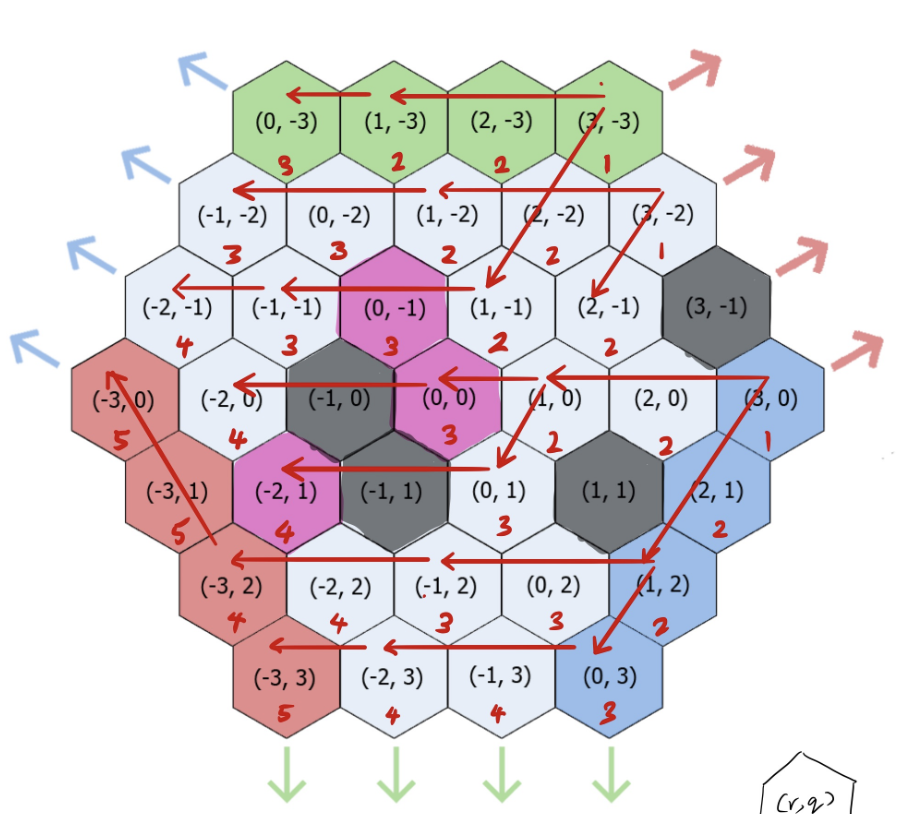
\includegraphics[width=0.3\textwidth]{heuristic.png}
                    \label{fig:heurstics}
                \end{center}
            \vspace{-10pt}
            \caption{Map formed by heuristic}
            \vspace{-100pt}
        \end{wrapfigure}
        \vspace{-40pt}
        \paragraph{Optimality} A* algorithm can only find the optimal solution if the heuristic is admissible. We relaxed the rule to allow pieces jumping freely without the need to leapfrog another piece. Because jump move allows pieces to move twice the normal move, our heuristic at most underestimates the real cost by a factor of $2$, and cannot be faster the real cost. This satisfied admissibility. Monotonicity is also met because each move adds $1$ unit of cost. Hence our program is optimal.
        \vspace{-10pt}
        \paragraph{Completeness} A* algorithm is complete if the graph contains finite nodes. For our problem, both the board and number of pieces are finite leading to a bounded size for state space, concludes the completeness of our algorithm.
    \section{Beyond}
    
        The complexity of problem is \textbf{exponentially} related to \textbf{number} of \textbf{moving pieces}. This is due to the effect of more moving options leading to a higher branching factor.\\
        The \textbf{further} pieces are from the \textbf{goal}, deeper the program has to search.\\
        A* algorithm stores each layer of nodes in a priority queue and only expend the $node$ $n$ with the $f(n)$. In the \textbf{worst case}, it expands all the nodes fully, store and sort them in order of cost, giving $O(b^d)$ complexity for both \textbf{space and time}. In the best case, our heuristic matches the real cost, and A only expand nodes with the correct path. This gives us $O(bd)$. The \textbf{high memory complexity} of A* ($O(b^d)$) can be avoided by using \textbf{iterative deepening A search}. This would reduce A* algorithm's \textbf{space complexity} to $O(bd)$ (by trading off some time complexity).\\
        The amount of free space on the board also affects the complexity of algorithm. From \ref{fig:moves} we can see that as the board becomes more empty, we have more actions to consider. Despite the low cost solution of \ref{fig:more_move}, its free space is drastically larger, leading to a significantly higher number of expanded nodes than that of \ref{fig:less_move}.
        \begin{wrapfigure}{r}{0.45\textwidth}
    \begin{center}
        \begin{subfigure}[b]{0.2\textwidth}
            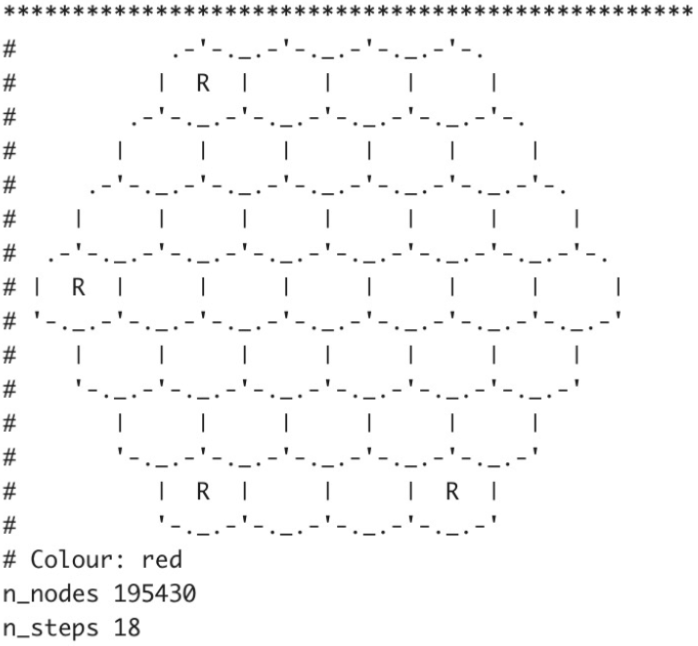
\includegraphics[width=\textwidth]{SpaceComplexity1.png}
            \caption{More options}
            \label{fig:more_move}
        \end{subfigure}
        \begin{subfigure}[b]{0.2\textwidth}
            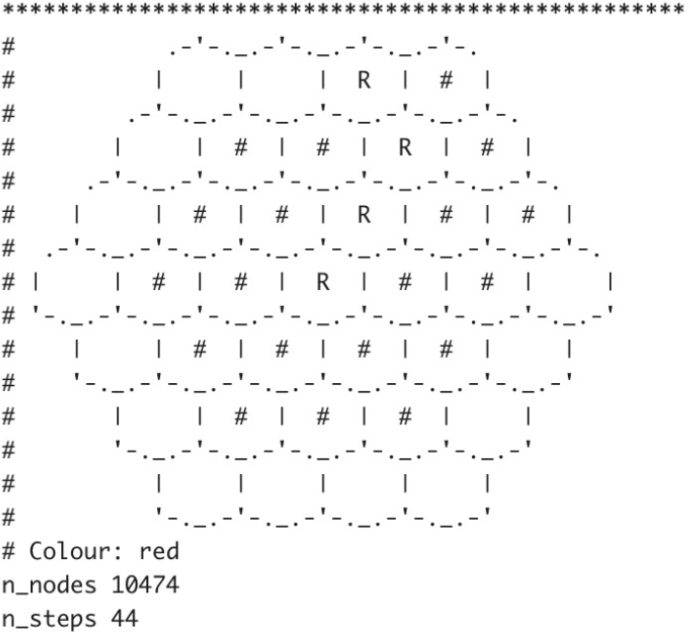
\includegraphics[width=\textwidth]{SpaceComplexity2.png}
            \caption{Less Options}
            \label{fig:less_move}
        \end{subfigure}
    \end{center}
    \vspace{-10pt}
    \caption{Search space illustration}\label{fig:moves}
\end{wrapfigure}
\end{document}
